% Task 4: one key, many messages. Values from Task4/one_key.py and Task4/rc4.py, CHECKED with python3:
%   rc4 keystream of b"our secret": b5 d0 d4 df ...
%   rc4(b"our secret", b"Meet at noon.") = f8 b5 b1 ab ..., rc4(b"our secret", b"Bring the map") = f7 a2 bd b1 ...
%   two example values of n (in the program they are random): 3b 91 e4 and c7 05 6a
%   keystream(n + key): f8 4a 4e 74 ... and e8 94 aa a2 ...
%   rc4(n + key, m1) = b5 2f 2b 00 ...,  rc4(n + key, m2) = aa e6 c3 cc ...
\documentclass[12pt,tikz,border=6pt]{standalone}
% Shared preamble of the task figures of Lecture 1.
% The colours and styles are copied from the preamble of ../main.tex (keep them in sync).
\usepackage{lmodern}
\usepackage[T1]{fontenc}
\renewcommand{\familydefault}{\sfdefault}
\usepackage{amsmath,amssymb}
\usepackage{xcolor}
\usepackage{fontawesome5}
\usetikzlibrary{arrows.meta, calc, positioning, fit, decorations.pathreplacing, decorations.pathmorphing, backgrounds}

% ---------- template ----------
\definecolor{DeepBlue}{HTML}{283593}
\definecolor{AccentOrange}{HTML}{EB5A14}
\definecolor{LightGray}{HTML}{F5F6FA}
% ---------- actors and categories (S1 to S6) ----------
\definecolor{sIndigo}{HTML}{5C6BC0}   % the sender
\definecolor{sPink}{HTML}{EC407A}     % the attacker
\definecolor{sViolet}{HTML}{7E57C2}   % plaintext
\definecolor{sAmber}{HTML}{FFB300}    % key and keystream
\definecolor{sTeal}{HTML}{26A69A}     % the receiver
\definecolor{sBrown}{HTML}{8D6E63}    % ciphertext
\definecolor{sPinkText}{HTML}{C2185B}
\definecolor{sAmberText}{HTML}{A06A00}
\definecolor{sTealText}{HTML}{00796B}
% ---------- actions and results ----------
\definecolor{aExec}{HTML}{43A047}
\definecolor{aRead}{HTML}{1E88E5}
\definecolor{aWrite}{HTML}{E53935}
% ---------- neutral ----------
\definecolor{nInk}{HTML}{37474F}
\definecolor{nLine}{HTML}{90A4AE}
\definecolor{nLight}{HTML}{CFD8DC}
\definecolor{nFill}{HTML}{ECEFF1}
\definecolor{nIdle}{HTML}{E0E0E0}

% ---------- TikZ styles (as in main.tex; byte cells a little larger for the web) ----------
\tikzset{
  hw/.style={draw=nLine, thick, fill=nFill, text=nInk, rounded corners=3pt, align=center, inner sep=4pt},
  hwmain/.style={draw=nInk, thick, fill=nInk, text=white, rounded corners=3pt, align=center, inner sep=4pt},
  cell/.style={draw=nLine, thick, fill=white, text=nInk, font=\ttfamily\small},
  cellfree/.style={cell, dashed, draw=nLight},
  container/.style={draw=nLine, thick, dashed, rounded corners=5pt},
  actor/.style={fill=#1, draw=#1, text=white, rounded corners=3pt, align=center, font=\small\bfseries, inner sep=5pt},
  actorlight/.style={fill=#1!15, draw=#1, thick, text=nInk, rounded corners=3pt, align=center, inner sep=5pt},
  data/.style={-{Stealth}, very thick, nInk},
  flow/.style={-{Stealth}, very thick, DeepBlue},
  annot/.style={draw=AccentOrange, line width=1.6pt, rounded corners=3pt},
  byte/.style={draw=nLine, thick, fill=white, text=nInk, font=\ttfamily\small,
    minimum width=0.8cm, minimum height=0.62cm, inner sep=1pt, rounded corners=1.5pt},
  ptb/.style={byte, fill=sViolet!15, draw=sViolet},
  ksb/.style={byte, fill=sAmber!25, draw=sAmber},
  ctb/.style={byte, fill=sBrown!15, draw=sBrown},
  unk/.style={byte, fill=white, dashed, text=sViolet},
  rowlabel/.style={font=\small\bfseries, text=nInk, anchor=east},
  note/.style={font=\small, text=nInk},
  bigxor/.style={circle, draw=nInk, very thick, fill=white, inner sep=0pt, minimum size=0.8cm, font=\Large},
  radio/.style={-{Stealth}, very thick, nInk, decorate,
    decoration={snake, amplitude=1.2pt, segment length=7pt, post length=4pt}},
  % a white card behind the whole figure, so that it stays readable in a dark theme
  card/.style={show background rectangle, background rectangle/.style={fill=white, draw=none}, inner frame sep=8pt},
}
% a row of bytes: \byterow{x of the first cell}{y}{style}{list of values}{step between cells}
\newcommand{\byterow}[5]{%
  \expandafter\def\expandafter\brlist\expandafter{#4}%
  \foreach \v [count=\k from 0] in \brlist {
    \node[#3] at ({#1+#5*\k},#2) {\v};
  }}
% the generator / cipher box: dark, with cogs. \cogbox{name}{position}{label}{width}
\newcommand{\cogbox}[4]{%
  \node[hwmain, minimum width=#4, minimum height=1.3cm] (#1) at (#2) {};
  \node[text=white, font=\Large] at ([yshift=0.22cm]#1.center) {\faCogs};
  \node[text=white, font=\small\bfseries] at ([yshift=-0.32cm]#1.center) {#3};}
\newcommand{\ok}{\textcolor{aExec}{\faCheck}}
\newcommand{\nok}{\textcolor{aWrite}{\faTimes}}
\newcommand{\badge}[1]{\tikz[baseline=(b.base)]\node[circle,fill=AccentOrange,text=white,
  inner sep=1.5pt,font=\bfseries\footnotesize] (b) {#1};}

\begin{document}
\pagecolor{white}
\begin{tikzpicture}[>=Stealth]
  \def\dx{0.85}
  \tikzset{nb/.style={byte, fill=white, draw=sAmber, line width=1.2pt}}
  % key -> RC4 -> keystream, on one row at height #1
  \newcommand{\keyrow}[1]{%
    \node[actorlight=sAmber, font=\small, minimum height=0.7cm] (k) at (4.75,#1) {\faKey\ \texttt{our secret}};
    \node[hwmain, minimum width=1.7cm, minimum height=0.75cm, font=\small\bfseries] (r) at (7.75,#1) {\faCogs\ RC4};
    \draw[data] (k) -- (r);
    \draw[data] (r.east) -- (9.05,#1);}
  \newcommand{\ksrow}[2]{\byterow{9.5}{#1}{ksb}{#2}{\dx}\node[text=nInk] at ({9.5+4*\dx-0.15},#1) {\ldots};}
  \def\cx{17.0}

  % ---------------- step 1 ----------------
  \node[font=\normalsize\bfseries, text=nInk, anchor=west] at (-0.4,1.45) {\badge{1}\ The same key for two messages};
  \node[font=\small\bfseries, text=sAmberText] at ({9.5+1.5*\dx},0.85) {keystream};
  \node[font=\small\bfseries, text=sBrown] at ({\cx+1.5*\dx},0.85) {ciphertext};
  \foreach \y/\m/\z/\c in {0.25/{m1 = Meet at noon.}/{B5,D0,D4,DF}/{F8,B5,B1,AB}, -0.75/{m2 = Bring the map}/{B5,D0,D4,DF}/{F7,A2,BD,B1}} {
    \node[note, anchor=east, font=\ttfamily\small] at (3.3,\y) {\m};
    \keyrow{\y}
    \ksrow{\y}{\z}
    \draw[data] (13.15,\y) -- node[above, font=\small, text=nInk] {XOR m} (16.45,\y);
    \byterow{\cx}{\y}{ctb}{\c}{\dx}
    \node[text=nInk] at ({\cx+4*\dx-0.15},\y) {\ldots};
  }
  \draw[annot] (9.0,-1.15) rectangle (13.0,0.65);
  \node[font=\small\bfseries, text=AccentOrange, anchor=north] at (11.0,-1.2) {the same keystream, as in Task 3};

  \draw[nLight, thick, dashed] (-0.4,-2.0) -- (20.6,-2.0);

  % ---------------- step 2 ----------------
  \node[font=\normalsize\bfseries, text=nInk, anchor=west] at (-0.4,-2.5) {\badge{2}\ A new public \texttt{n} for every message. The RC4 key is \texttt{n + key}.};
  \node[font=\small\bfseries, text=nInk, align=center] at (1.0,-3.3) {\texttt{n}: 3 random bytes (example)};
  \node[font=\small\bfseries, text=sAmberText] at ({9.5+1.5*\dx},-3.3) {keystream};
  \node[font=\small\bfseries, text=nInk] at ({\cx-0.4},-3.3) {packet sent: \texttt{n + c}};
  \foreach \y/\n/\z/\c in {-3.95/{3B,91,E4}/{F8,4A,4E,74}/{B5,2F,2B,00}, -4.95/{C7,05,6A}/{E8,94,AA,A2}/{AA,E6,C3,CC}} {
    \byterow{0.15}{\y}{nb}{\n}{\dx}
    \node[font=\large\bfseries, text=nInk] at (2.85,\y) {+};
    \keyrow{\y}
    \ksrow{\y}{\z}
    \draw[data] (13.15,\y) -- (14.0,\y);
    \byterow{\cx-2.55}{\y}{nb}{\n}{\dx}
    \byterow{\cx}{\y}{ctb}{\c}{\dx}
    \node[text=nInk] at ({\cx+4*\dx-0.15},\y) {\ldots};
  }
  \draw[annot] (9.0,-5.35) rectangle (13.0,-3.6);
  \node[font=\small\bfseries, text=AccentOrange, anchor=north] at (11.0,-5.4) {a new \texttt{n} gives a new keystream};
  \node[font=\small, text=nInk, anchor=north west] at (14.0,-5.4) {\texttt{n} travels in the open, the key stays secret};
\end{tikzpicture}
\end{document}
